\subsection{Manager Pages}
\par \noindent The first page that the manager can see, after logging in, is his homepage, where he sees an overview of the latest news, such as the number of new bookings or a list with the currently bookings and their relative details, and a list with the last accesses of the front office users.
\par \noindent In the booking history, the manager can navigate through an accordion list of all the rooms, and see, for each of them, some details about the bookings in that room. The manager can click on a room's name and all the details appeared: an overview of the room's booking is shown, and two tables that show the information about of currently and soon bookings. For each room, the manager can download a log file.
\par \noindent In the payments page, the manager check information about the payments. A first table shows a list of pending payments with relative details, and a second table shows a list of confirmed payments with relative details. For both of them a log file can be downloaded.
\par \noindent The users page is divided into two area. In the first one, the manager can compile a form and add a new front office user. In the second one, a table shows a list of all the front office users with relative details and relative buttons to manage them: there is a button that allows the manager to edit the details of the users (e.g., email), another button that allows to send reset password link, and in the end there is another button to delete the user from the system.
\par \noindent The last one page, called "add booking", shows the procedure to add a booking of a customer. In the case the customer does not book online but physically on the hotel, the manager can proceede with the booking from this interface.
% list of all the images of the manager area

\begin{figure}[H]
	\centering
	%\label{fig:manager-index}
	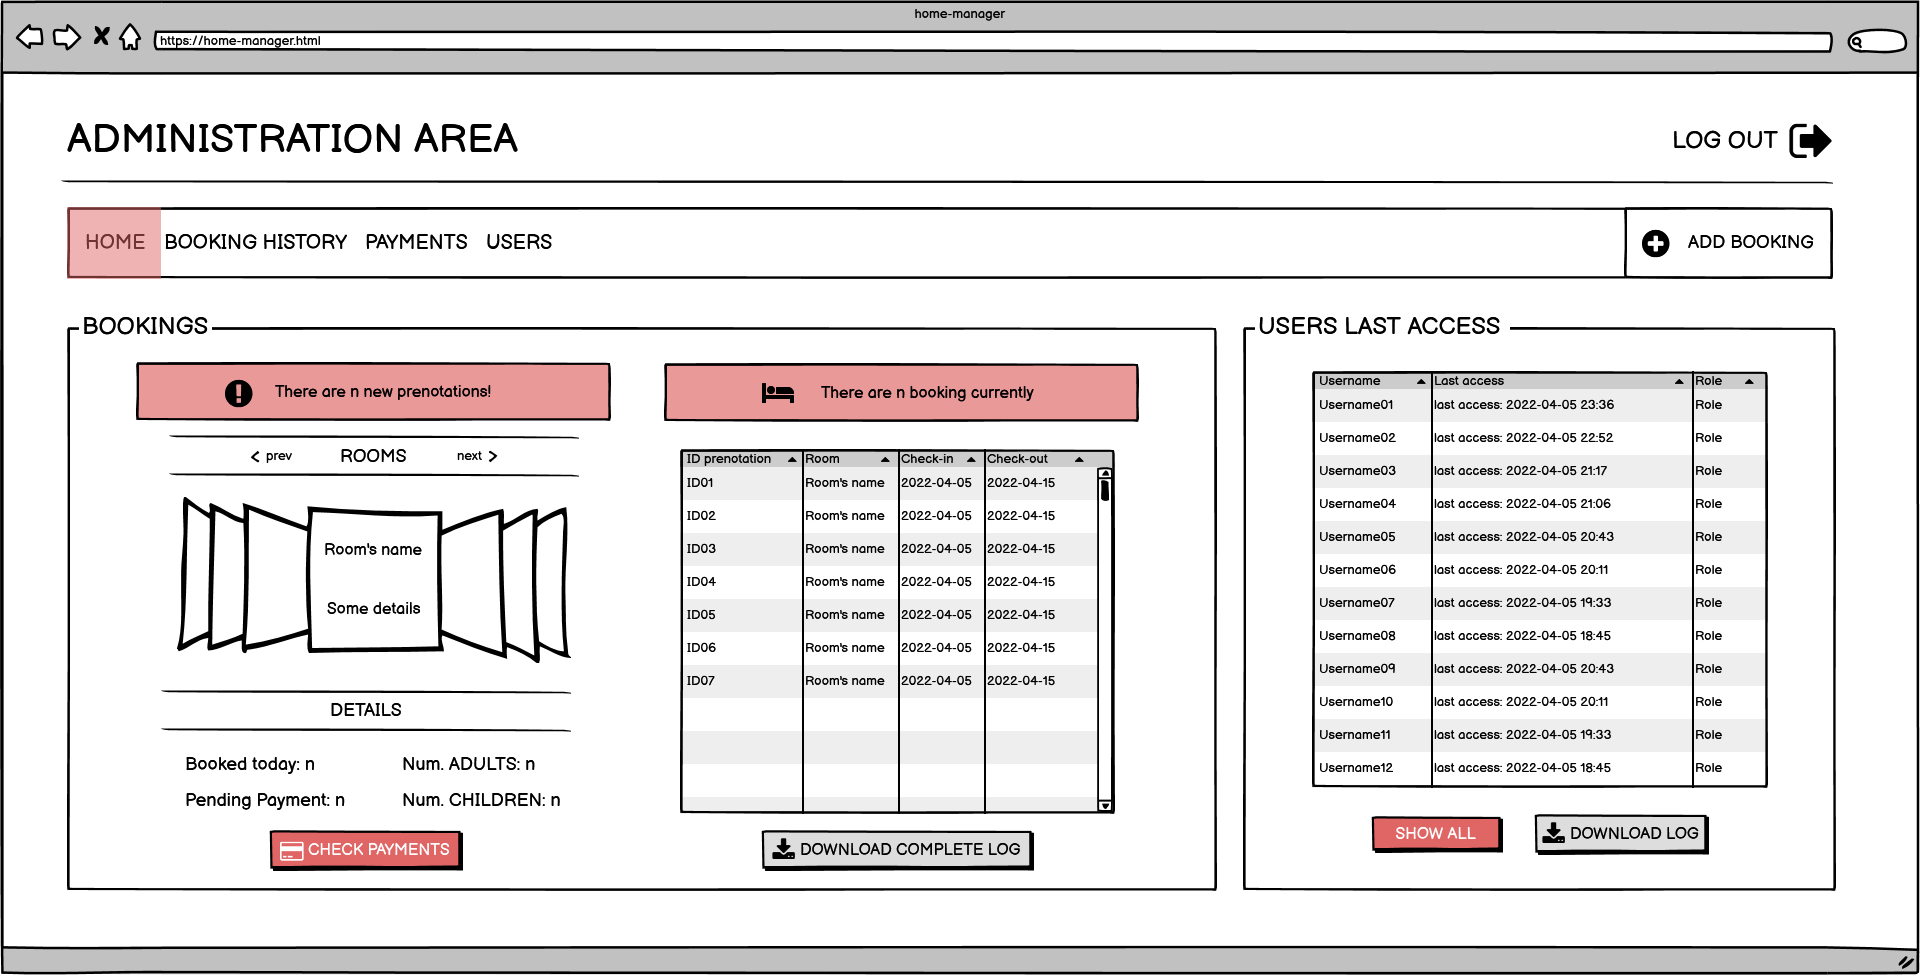
\includegraphics[height=7.5cm]{images/manager-index.png} 
	\caption{Administration area: Manager homepage}
\end{figure}
\begin{figure}[H]
	\centering
	%\label{fig:manager-index}
	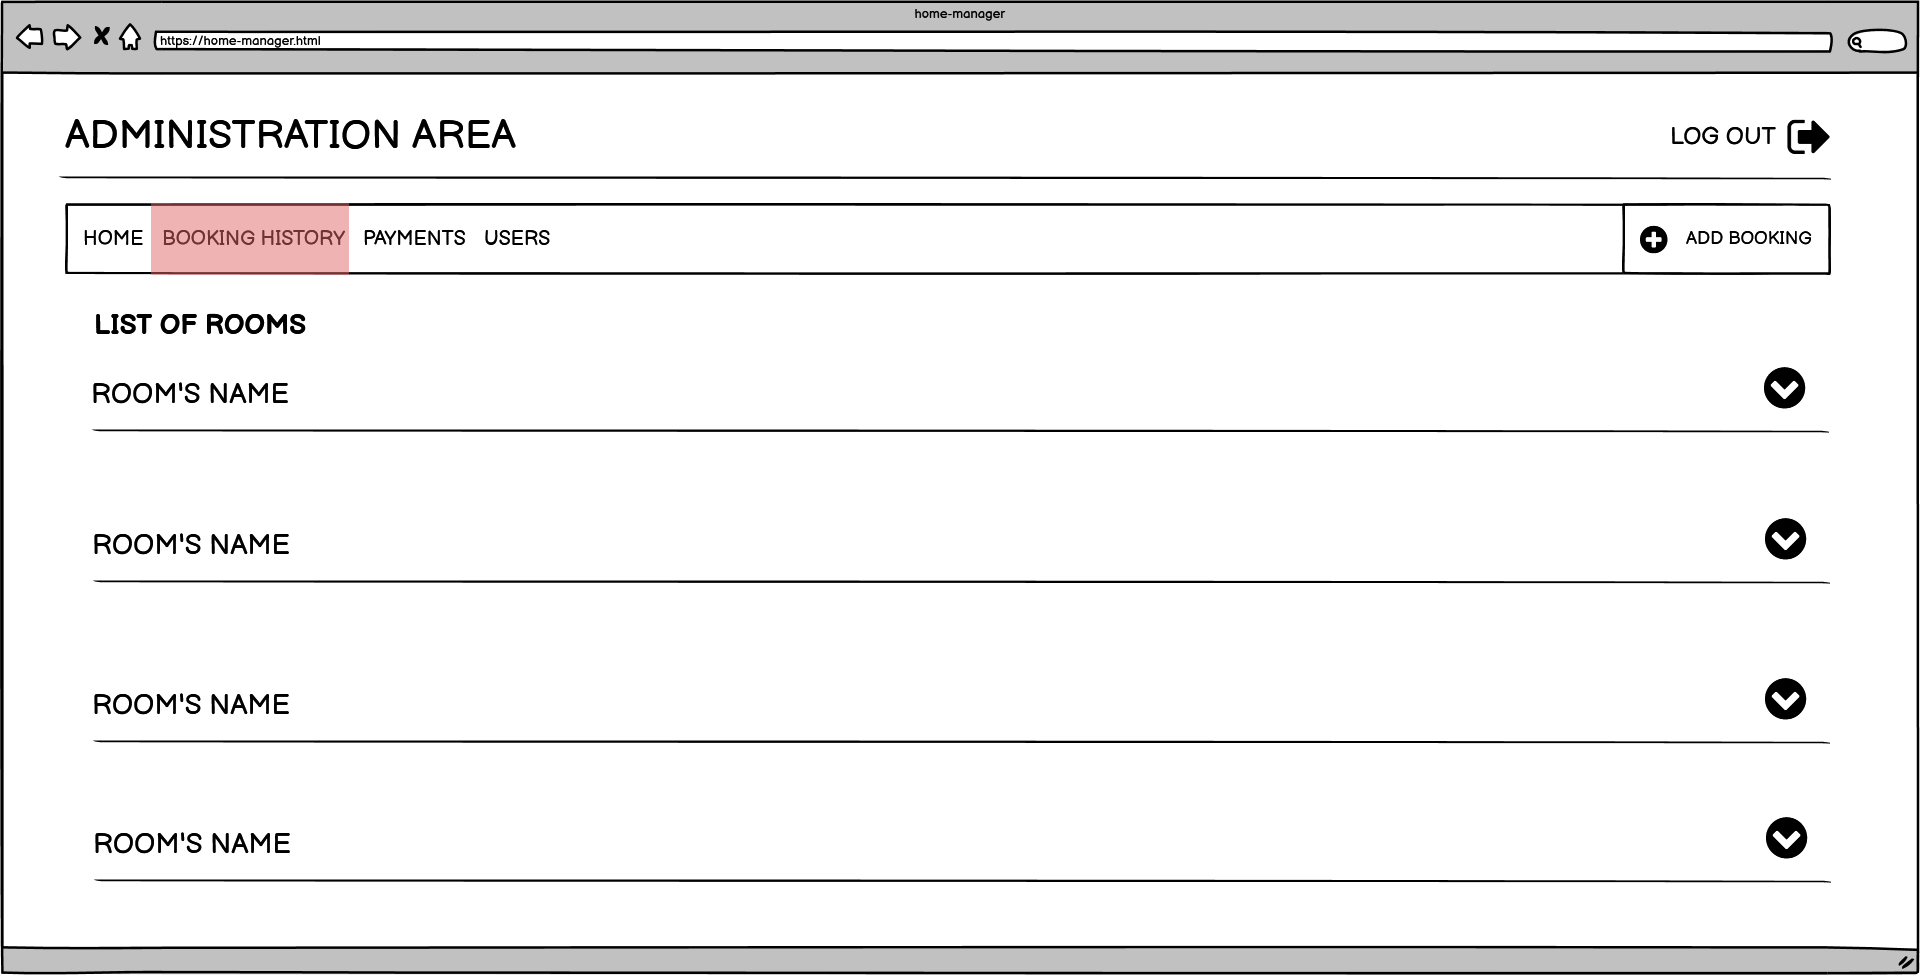
\includegraphics[height=7.5cm]{images/admin-booking-hist.png} 
	\caption{Administration area: Booking history page}
\end{figure}
\begin{figure}[H]
	\centering
	%\label{fig:manager-index}
	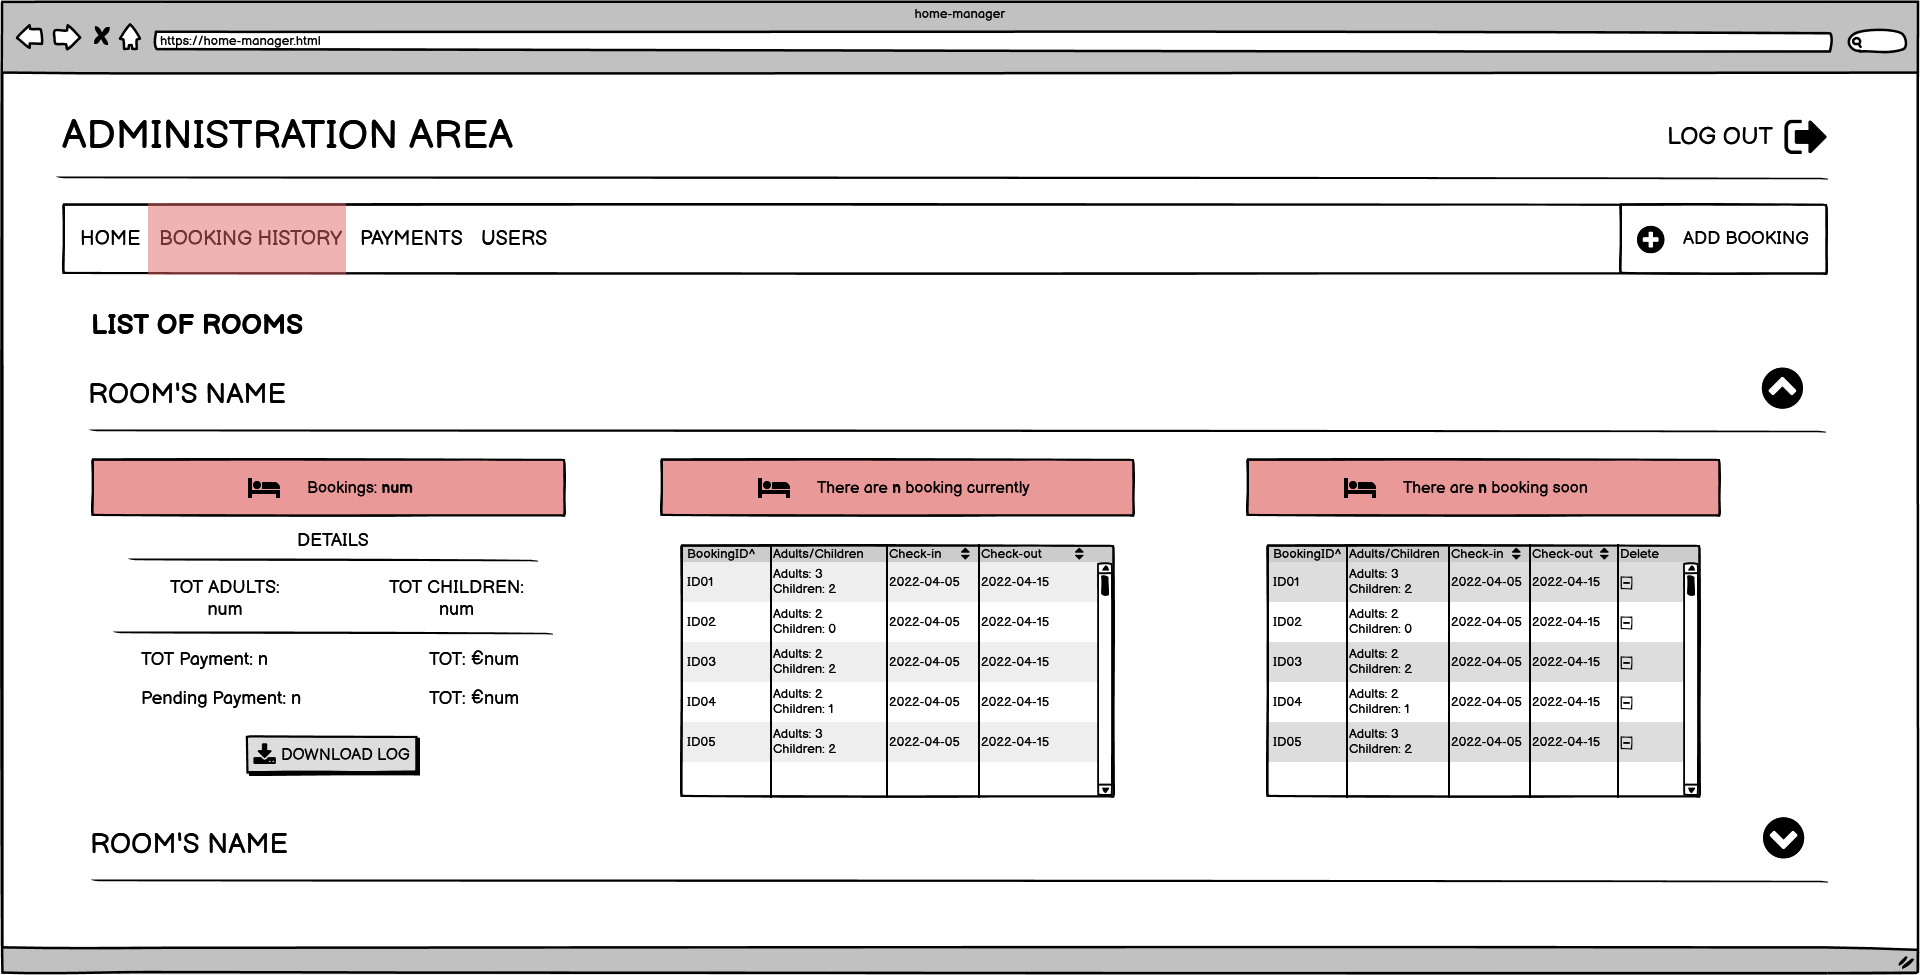
\includegraphics[height=7.5cm]{images/admin-details-room.png} 
	\caption{Booking history page: the room's details}
\end{figure}
\begin{figure}[H]
	\centering
	%\label{fig:manager-index}
	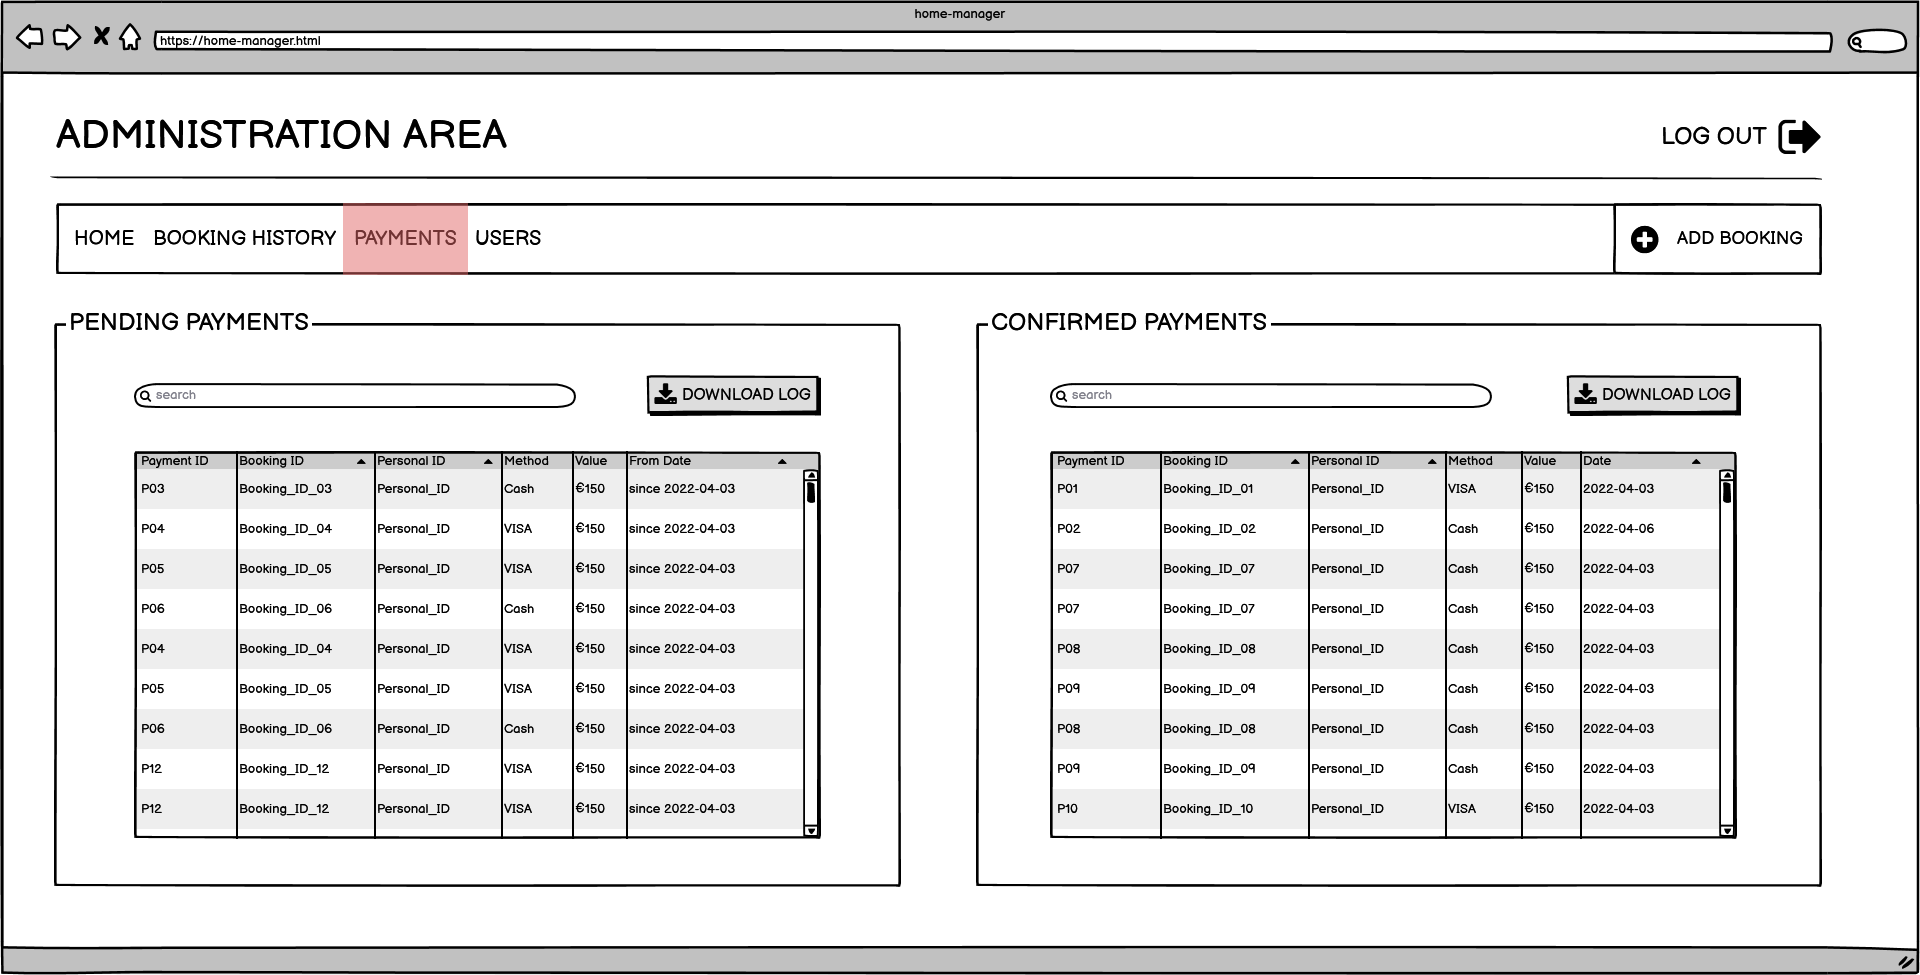
\includegraphics[height=7.5cm]{images/manager-payments.png} 
	\caption{Manager area: Payments page}
\end{figure}
\begin{figure}[H]
	\centering
	%\label{fig:manager-index}
	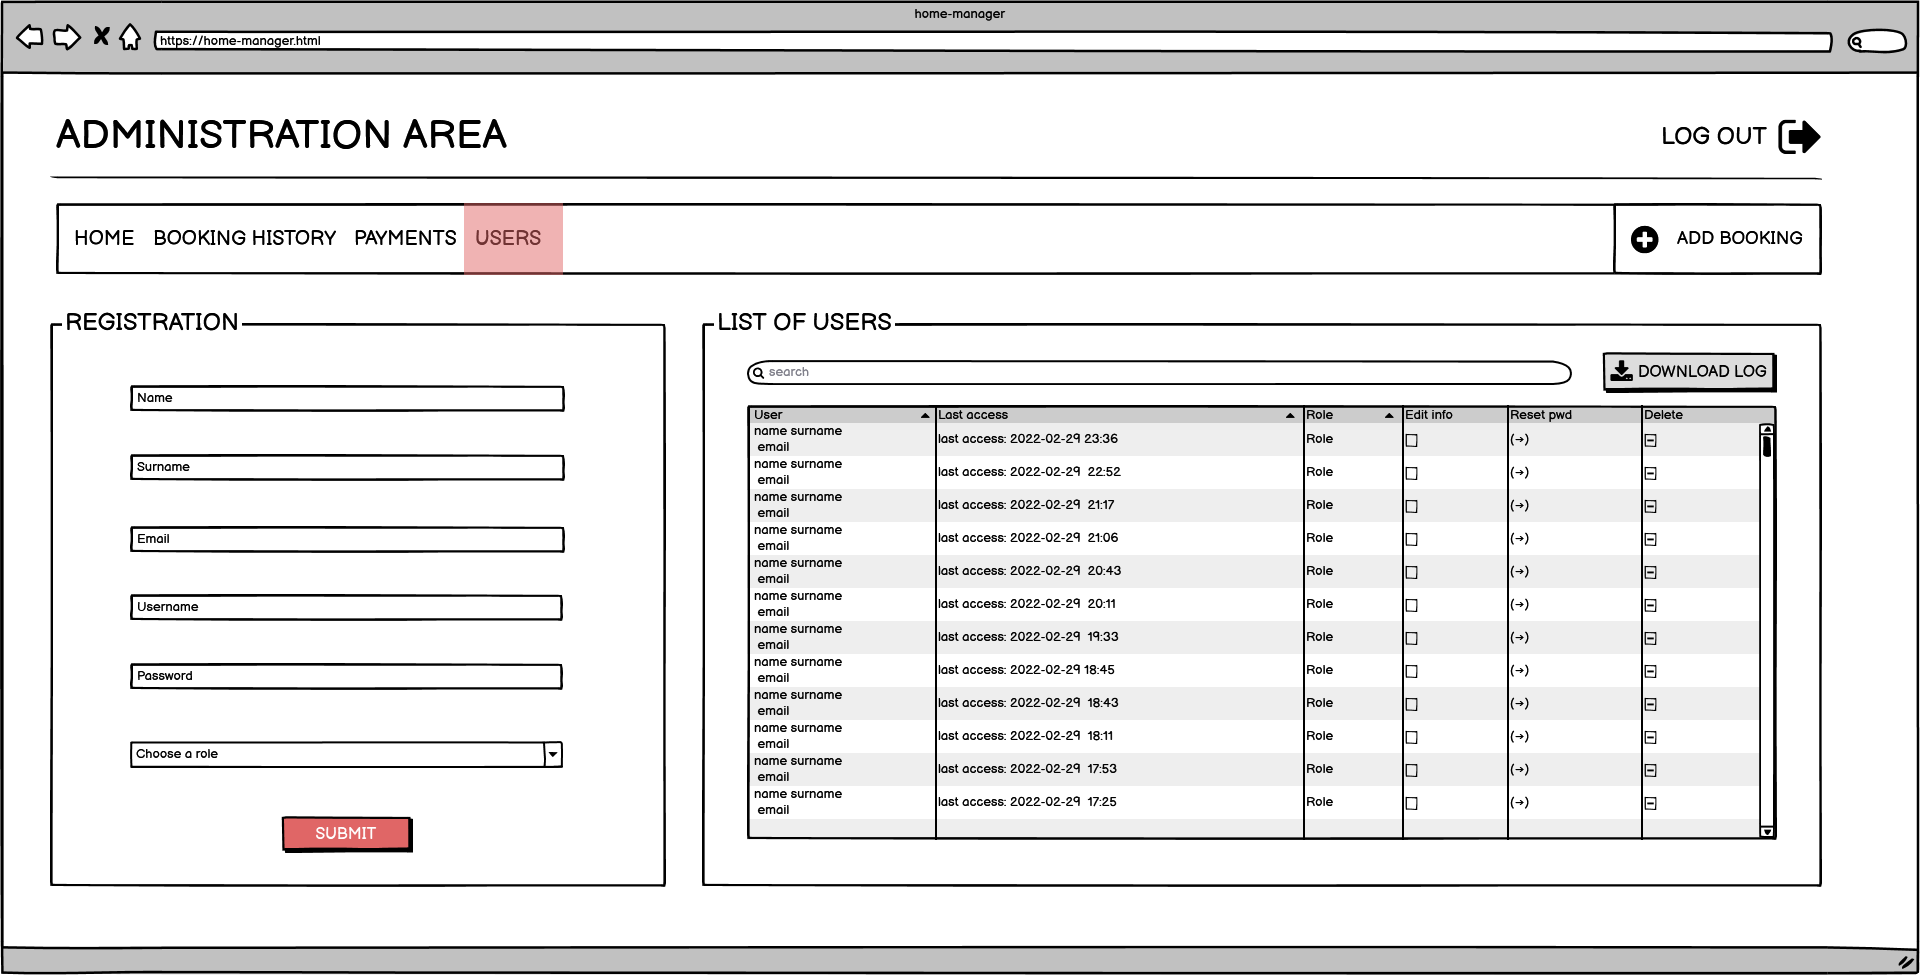
\includegraphics[height=7.5cm]{images/manager-users-page.png} 
	\caption{Manager area: Users management page}
\end{figure}
\begin{figure}[H]
	\centering
	%\label{fig:manager-index}
	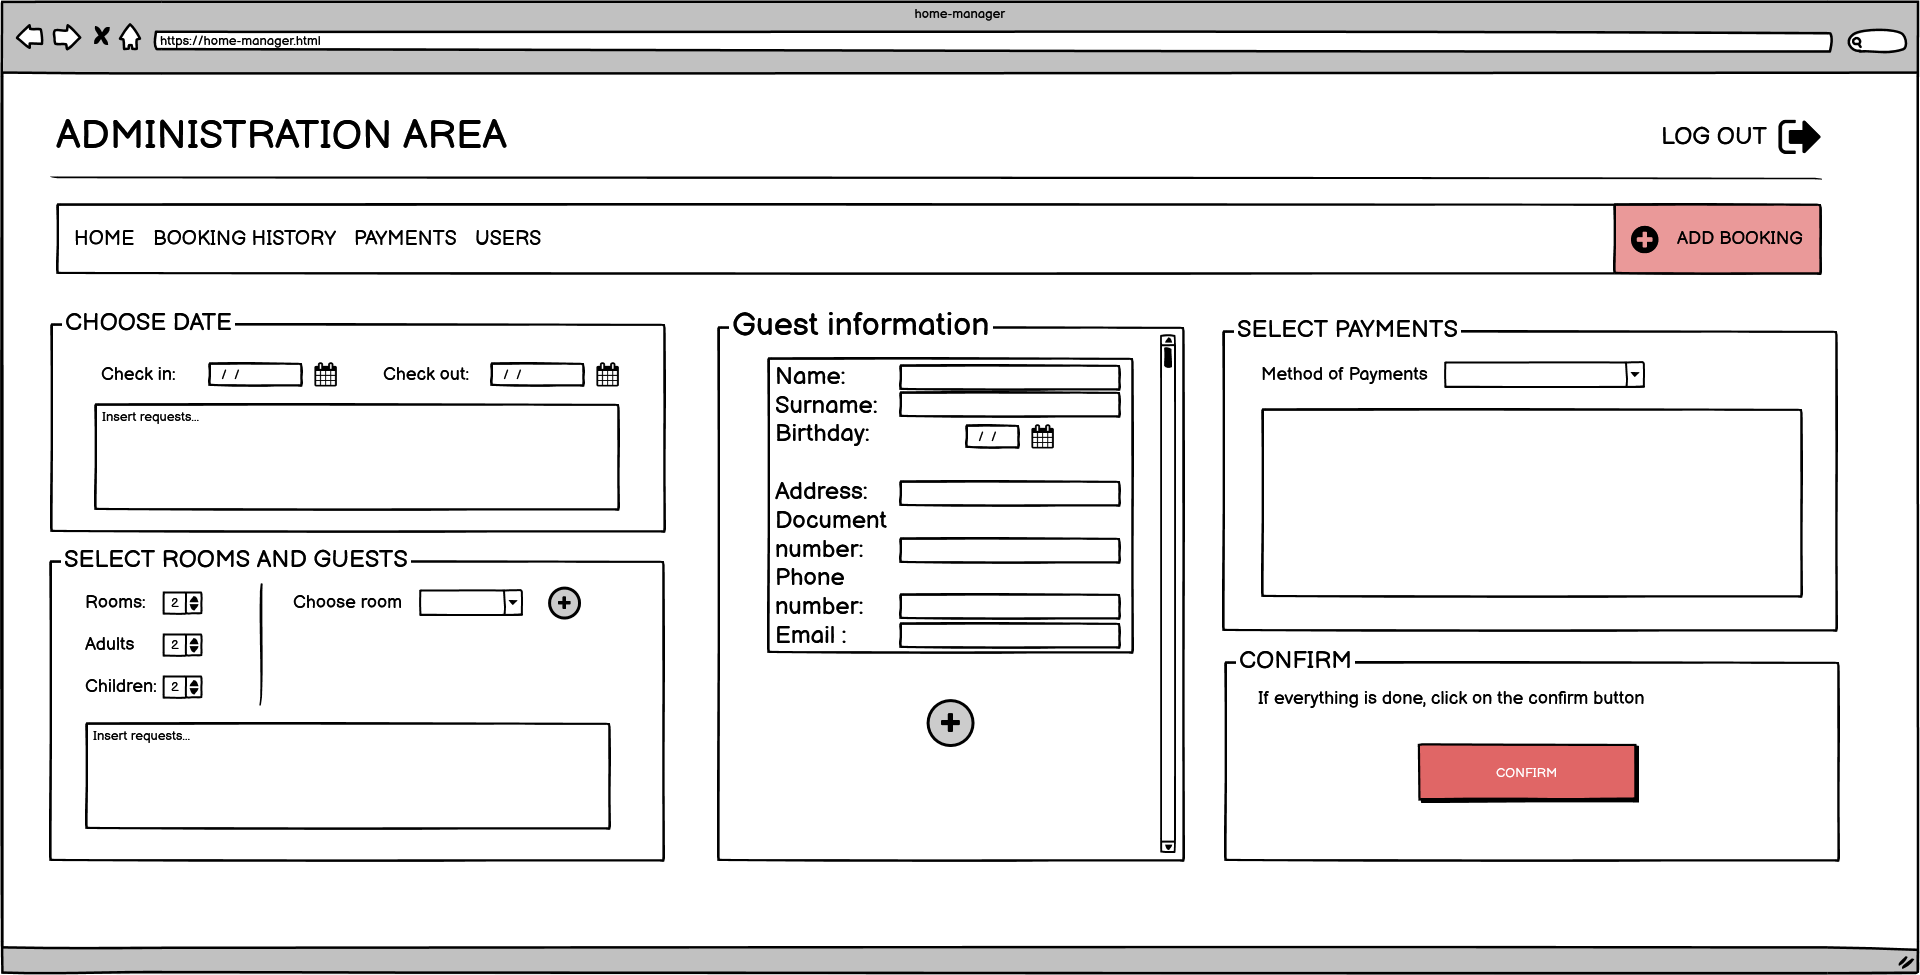
\includegraphics[height=7.5cm]{images/admin-add-books.png} 
	\caption{Administration area: Add bookings page}
\end{figure}